
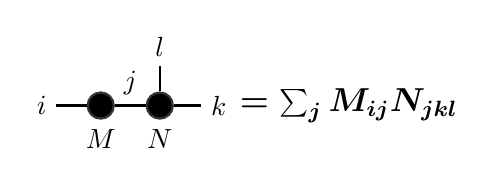
\begin{tikzpicture}
	\node[circle,draw=black!80,thick,fill=black,label=below:$M$] (M) at (0.75,0) {};
	\node[circle,draw=black!80,thick,fill=black,label=below:$N$] (N) at (1.5,0) {};
	\node (i) at (0,0) {$i$};
	\node (l) at (1.5,0.75) {$l$};
	\node (k) at (2.25,0) {$k$};
	\draw[thick, draw=black,label=above:] (M) -- node [above] {$j$} (N) {};
	\draw[thick, draw=black] (i) -- (M) {};
	\draw[thick, draw=black] (N) -- (k) {};
	\draw[thick, draw=black] (N) -- (l) {};
	\node at (3.9,0) {\large {\boldmath$= \sum_j M_{ij}N_{jkl}$}};
\end{tikzpicture}
